\section{Ecossistema de software}

% ecossistema pode estar organizado em relacões de benefício mútuo

Ecossistema de software é definido, segundo \citeonline{manikas2013software},
como a interação entre diversos atores numa plataforma tecnológica comum
resultando em novas soluções de softwares ou novos serviços. Cada ator neste
sistema é motivado por um conjunto de interesses e conectam-se entre si e ao
próprio sistema numa relação simbiótica, fazendo a plataforma tecnológica
evoluir enquanto permite o envolvimento e contribuição de novos e diferentes
atores.

Nesta relação os atores são beneficiados de formas diferentes dependendo da
natureza do ecossistema, num ambiente comercial, por exemplo, os atores ganham
receita financeira diretamente (salário, prêmios, etc), enquanto num sistema
não-comercial os atores estão motivados por questões não-monetários (fama,
conhecimento, ideologia, etc).

De uma forma ou de outra, todos são beneficiados, os atores e o próprio
ecossistema, os atores recebem mais (ou melhores) benefícios com o crescimento
do ecossistema, o ecossistema oferece cada vez mais (ou melhores) benefícios
com as atividades dos seus atores, resultando numa relação de benefício
mútuo.

Este modelo geral de funcionamento do ecossistema de software pode variar a
depender do contexto em que se insere, o ecosistema de software acadêmico por
exemplo possui a particularidade de estar inserido no sistema de reputação
científica de alguma forma.

%possibilita esse tipo relação simbiótica
%apesar de não determinar que todo ecossistema aproveite tal benefício.
%
%Adicionalmente as relacões entre os atores do ecosistema como um todo
%são de mútuo interesse (mutualismo):
%
%O relacionamento entre os atores em um ecossistema de software, por outro lado,
%são caracterizados pela alto espectro de relacionamentos simbioticos.
%
%Dependendo dos atores e suas atividades, dois atores podem ter benefícios
%mútuos (mutualismo), estar em competição direta (competition/antagonism),
%estarem não afetados (neutralism) ou um não afetado enquanto o outro é
%beneficiado (amensalism) ou prejudicado (parasitism) por seu relacionamento

\section{Ecossistema de software acadêmico}

% , traduzido para software acadêmico para evitar o
% termo {\it software de pesquisa}, a palavra {\it research} em português {\it
% pesquisa} pode ser facilmente confundida com ferramentas ou sistemas de
% pesquisa, como sites de pesquisa por exemplo,

O ecossistema de software acadêmico possui a particularidade de estar inserido
num contexto que se relaciona com a economia de reputação científica,
especialmente com o sistema de publicação, sendo influenciado e influenciando
diretamente o impacto causado pelas suas publicações e pelo seu sistema de crédito
acadêmico.

% (5) Tools in mining software repositories \cite{chaturvedi2013tools}
% Faz uma revisão dos papers submetidos ao MSR desde 2007 até 2013 (?) e
% identifica data sets, ferramentas e técnicas utilizadas pelos autores, mais
% da metade dos papers usam ou criam ferramentas, categoriza as ferramentas em
% ferramentas novas, ferramentas tradicionais, protótipos e scripts para
% mineração de dados

\citeonline{howison2015understanding} criou um framework para pensar e refletir
sobre o processo de produção de softwares na ciência, e identificou quatro
papéis envolvidos no ecossistema de softwares acadêmicos, cientistas usuários
finais, produtores e distribuidores de software, administradores de
infraestrutura e pesquisadores preocupados com o funcionamento do ecossistema
como um todo.

%Unlike other technologies supporting science, software can
%be copied and distributed at essentially no cost, potentially
%opening the door to unprecedented levels of sharing and col-
%laborative innovation. \cite{howison2011scientific}
%
%While some of these seem relatively unproblematic, such as commercial
%production in fields with immediately valuable applications, others appear
%problematic. In particular we highlighted the potentially pernicious
%implications of the academic credit production system for collaboration and
%maintenance.

\subsection{Cientistas usuários finais}

Pesquisadores de todos os domínio da ciência ocupam um papel chave no
ecossistema de software acadêmico, em seus processos de investigação e
experimentação fazem uso de artefatos de software para coletar, gerenciar,
transformar, analisar, modelar e visualizar os seus dados, sempre com o
objetivo final de publicar os seus resultados na literatura acadêmica.

Os cientistas estão preocupados com a disponibilidade, qualidade e usabilidade
destes artefatos de software e também com a capacidade de continuar úteis
podendo ser utilizados em conjunto com outros softwares. Estão interessados
também em saber o que outros cientistas usam em suas pesquisas, softwares com
alta adoção no domínio em que estão inseridos costumam manter os pesquisadores
mais livres e com maior foco em suas próprias pesquisas.

Uma alta adoção costuma ser sinal de uma boa qualidade de software, além
garantir que o grupo de pesquisa, estudantes e colaboradores consigam encontrar
mais facilmente o software e também obter ajuda entre os seus pares para
resolver questões sobre o uso do softare, simplifica também o trabalho dos
revisores pois encontrarão as mesmas facilidades no uso.

\subsection{Produtor e distribuidor de software acadêmico}

Um segundo papel é o que produtor de softwares acadêmicos, e distribuição. Varia
de indivíduos a times, ambos chamado de projetos para facilidade, produzindo
artefatos que são usados por pequenos grupos ou disciplinas inteiras.

Alguns softwares são desenvolvidos e muitas vezes ficam confinados em seus laboratórios
ou grupos, mas eventualmente são compartilhados e potencialmente amplamente adotados, tornando
o cientista parte do ecosistema do software (Van de Geijin 1997).

Muitas vezes são desenvolvidos em colaborações próximas entre cientistas de computação e
outras áreas, eles desenvolvem algoritmos que refletem as pesquisas dos pesquisadores
do domínio em questão. Um desafio é abstrair os problemas e implementar soluções que
podem ser adotadas por outros cientistas, especialmente em outros domínios.

Projetos se preocupam com o impacto cientifico tanto em termos de numero quando
tipo de usuários seu software atinge, e como seus softwares contribuem para a
ciencia que outros estão realizando.

Alguns projetos são gerenciados no estilo de código aberto, e tem
atraido com sucesso contribuições de muitos cientistas, incluindo
uma calda longa de contriuição que tem feito pequenas mas substanciais
contribuições.

\subsection{Provedor de infraestrutura}

Um terceiro papel é quem provê um cojunto de softwares que são
disponíveis aos usuários finais em seus trabalhos de pesquisa.
Este papel pode ser desempenhado como ciberinfraestrutura de software
em centros de supercomputação através de provedores de computação
em nuvem ou podem ser distribuidos, podem ser disponiveis para usuarios
fazer download em seus computadores pessoais.

Do ponto de vista de ecosistema, ambos os tipos de distribuiça
estão interessados nas mesmas questões: quem usa, ou não usa?
Qual versão usa? Em qual frequencia atualiza?

\subsection{Pesquisador}

Um último papel é daqueles preocupados sobre o funcionamento do
próprio ecosistema e sua contribuição para a ciência.

Costuma ser agencias de financiamento mas pode ser também cientistas sênior do
domínio que refletem além de seu trabalho individual e pensam em seus campos
como um todo.

As preocupações rondam ao redor de questões sobre operação do ecosistema como
um sistema que toma recursos (tempo, dinheiro e atenção) e afeta a conduta da
ciência, tanto o geral como em campos individuais, complementado pelo interesse
de saber como o comportamento desse sistema pode ser influenciado.

%Essas preocupações gerais sugerem um conjunto de questões específicas, com foco
%em padrões globais e padrões emergentes dentro do ecossistema, incluindo: Quais
%recursos foram destinados à produção de software? Quantos usuários ou
%comunidades de usuários têm projetos? Quais são os impactos científicos desse
%uso? Os números de usuários crescem? Os projetos possuem recursos e habilidades
%suficientes para gerenciar seu crescimento? Quais projetos possuem
%funcionalidades sobrepostas? Há quanto tempo os pedaços de software e projetos
%persistem? Nós desconectamos as comunidades de usuários e desenvolvedores? São
%componentes específicos, ou camadas de componentes, faltam? Que código
%geralmente é usado em conjunto; são os projetos e as pessoas que produzem esses
%componentes se comunicando adequadamente? Como podemos sustentar o software
%crítico?

Junto com estas questões estão as questões de como influenciar o ecossistema,
incluindo questões de pontos de inflexão que levam ao uso coalescente, bem como
a intervenções políticas diretas incentivando o uso de componentes específicos.

%Aqui há uma clara tensão entre um desejo de flexibilidade e liberdade, ligado
%às expectativas de inovação científica e desejos de estruturas de autoridade e
%controle de coordenação. As questões de influência incluem: como os programas
%de financiamento e quais os requisitos em suas chamadas, resultaram em software
%amplamente utilizado e impacto científico substancial? Quais são as
%características dos campos que alcançaram maior coalescência? Quais jornais e
%conferências têm políticas exemplares? Como o trabalho de software é visto
%dentro das práticas de contratação e avaliação, como os casos de posse?
%
%\cite{howison2015understanding}

\section{Modelo de produção de software acadêmico}

% recurso, uso e impacto

%Computer systems research spans sub-disciplines that in-
%clude embedded and real-time systems, compilers, network-
%ing, and operating systems. Our contention is that a number
%of structural factors inhibit quality research. We highlight
%some of the factors we have encountered in our work and ob-
%served in published papers and propose solutions that could
%both increase the productivity of researchers and the quality
%of their output \cite{Vitek2011}.

Figura \ref{process-model-scientific-software} apresenta um modelo simplificado 

\begin{figure}[h]
  \center
  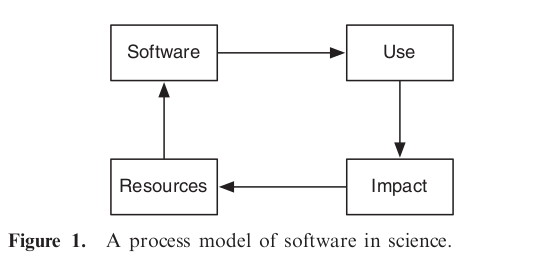
\includegraphics[scale=0.5]{imagens/process-model-scientific-software.png}
  \caption{A process model of software in science \cite{howison2015understanding}}
  \label{process-model-scientific-software}
\end{figure}


Estes atores participam do ecossistema dentro de seus próprios interesses, mas
sempre causando um impacto de volta no sistema, os usuários finais cientistas
(diretamente ou indiretamente) usam softwares acadêmicos para fazer ciência,
resultando em impacto científico, este impacto científico então justifica
investimento de novos recursos, que faz o ecossistema crescer fazendo os softwares
existentes evoluirem ou criando novos softwares.

%seja para fins de planejamento ou reflexão
%seja como retrospectiva para avaliar investimentos realizados.
%
%Recursos são devotados para a produção de software acadêmico. Usuários finais
%cientistas (diretamente ou indiretamente) usam softwares acadêmicos para fazer
%ciência, resultando em impacto científico. Impacto científico então justifica
%investimentos e recursos, seja de forma antecipada para fins de planejamento,
%seja como retrospectiva para avaliar investimentos realizados.

Compreender como os softwares acadêmicos vem a ser criados é um primeiro
passo crucial para avaliar seu .... quem faz, o quê, e quando?

\subsection{Recursos}

Cinco modelos de produção de software na ciência, distinguidos principalmente
pela motivação principal: (1) ganho monetário direto (comercial software,
employed software developers), (2) reputação acadêmica (incidental software,
dirigido pela necessidade científica direta), (3) prática de software paralela
(scientific needed enhanced by publishing 'software papers' alongside domain research),
(4) um software de uma subárea de pesquisa (reputação direta pelo trabalho do software),
(5) híbridos como licença-dual e 'software work' dentro de grandes colaborações
(software como uma contribuição científica direta).

Os recursos investidos na produção de software acadêmico vem de diversas
fontes, incluem ganhos monetários diretos, recurso alocado em projetos,
colaboração em 'service work', e ostensivamente 'tempo livre' dos pesquisadores
em busca de soluções em suas pesquisas, que perpassa financiamentos diversos,
carreira individual do cientista, estudantes de graduação, prêmios, etc.

O desenvolvimento de software acadêmico, assim como de qualquer outro
software, exige conhecimento sobre o domínio de aplicação, o que torna o
seu desenvolvimento essencialmente diferente é que este conhecimento pode ser,
por exemplo, entender como o DNA genômico se transforma em cristais de
proteína, ou os meandros da dinâmica dos fluidos, ou como resolver 20 equações
diferenciais parciais simultâneas \cite{segal2008developing}.

Isto faz com que os próprios cientistas acabem desenvolvendo os seus softwares,
um estudo entre cientistas do reino unido mostrou, por exemplo, que 56\%
desenvolvem seus próprios softwares, pelo menos pacialmente
\cite{hettrick_2014_14809}, outro estudo similar mostrou que na astronomia este
número chega a 90\% \cite{momcheva2015software}.

\subsection{Uso}

% ... software é distribuido, utilizado e dá suporte à ciencia, gerando impacto ...

Software acadêmico ({\it academic software}) é todo software usado para
coletar, processar ou analisar resultados de pesquisas com intenção de ser
publicados na literatura academica (seja num jornal, revista, conferência,
monografia, livro ou tese), podem ser desde protótipos escritos pelos próprios
cientistas, até mesmo produtos completos desenvolvidos profissionalmente
\cite{allen2017engineering}.

Estes softwares são usados ativamente em diversos campos de pesquisa, como
matemática, biologia, física de partículas, astronomia, medicina e direito,
eles resolvem problemas comuns do cotidiano de pelo menos metade dos
pesquisadores de todas as áreas, desde grupos trabalhando exclusivamente com
problemas computacionais até grupos em laboratórios tradicionais ou em campo
\cite{wilson2014best}.

Este uso causa impacto científico ... através do sistema de reputação acadêmica.

\subsection{Impacto científico}

% ... impacto científico justifica e potencialmente gera mais recurso ...

O impacto científico gerado pelo uso dos softwares acadêmicos está
entrelaçado com o sistema de crédito científico de suas publicações,
o sistema de publicação científico através de citações dá crédito ao
trabalho realizado, este sistema tem peomovido o avanço da ciência
mesmo diande de problemas para citação formal de artefatos digitais,
como são os softwares.

Apesar disso o impacto causado se reverte potencialmente em mais
recursos que poderão ser reinvestidos no próprio ecossistema onde
o software está inserido.

%historia da citacao na ciencia, como isso promove o avanço, problemas para
%citacao em artefatos digitais, solucao para identificador unico de autores de
%artigos, orcid.org resolve este problema, o mesmo para identificar artefatos
%digitais é o doi.org \cite{allen2014credit}.

%%%%%%%%%%%%%%%%%%%%%%%%%%%%%%%%%%%%%%%%%%%%

No entanto tem se percebido que o ecossistema de software acadêmico tem perdido
oportunidade de colaboração visto que estão inseridos neste contexto ....
competição, muitos softwares utilizados em pesquisas não são mencionados
pelos seus autores causando impacto negativo em sua visibilidade, reconhecimento e
consequentemente ...  \cite{howison2016software}.

%A comunidade tem refletido sobre os problemas relacionados ao
%desenvolvimento, promoção e sustentabilidade desses softwares, e o
%impacto que tais problemas causam no meio científico \cite{allen2017engineering}. Esta
%reflexão tem mostrado, por exemplo, que muitos estudos em engenharia de
%software sofrem de dificuldades de repetição \cite{Tang2016}, e apontam
%problemas específicos relacionados à manutenabilidade e a sustentabilidade
%técnica dos softwares acadêmicos.

\section{Problemas no ecossistema de software acadêmico}

% problemas identificados no ecossistema de software acadêmico

%\subsubsection{Desenvolvimento}

O {\it Dagstuhl Perspective Workshop} é um evento organizado por e para um
pequeno grupo de pesquisadores sêniores de renome internacional, realizado
anualmente na universidade de Dagstuhl\footnote{\url{http://www.dagstuhl.de}}
com o objetivo de refletir sobre o atual estado da ciência da computação.

%Através de uma discussão intensiva com foco estratégico o workshop explora
%tópicos novos e emergentes da ciência da computação produzindo manifestos que
%capturam tendências e desenvolvimentos relacionados aos tópicos explorados.
%
%Realizado desde 2011 o workshop tem explorado diversos tópicos da ciência da
%computação, como computação e paleografia, tecnologia da informação como ponte
%entre biologia e medicina, métodos de aprendizado de máquina para segurança de
%computadores, análise de performance e visualização, entre outros tópicos.

Em sua mais recente edição, o Dagstuhl Perspectives Workshop on ``Engineering
Academic Software'' \cite{allen2017engineering} examinou o estado atual dos
softwares acadêmmicos, identificou problemas comuns em seu desenvolvimento,
reconhecimento e sustentabilidade.

%Uma das contribuições chave deste workshop é um manifesto contendo um roteiro
%para o futuro da engenharia de software profissional e acadêmica, com foco em
%instrumentos de suporte para pesquisas em software científico. O manifesto é
%expresso em termos de ações ``promessas'' destinado a usuários e
%desenvolvedores de softwares científicos, com passos concretos para melhorar o
%ambiente em que os softwares são produzidos.
%
%Os compromissos expressados neste manifesto são agrupados em três conceitos gerais:
%(i) garantir que softwares científicos sejam {\it citados} apropriadamente;
%(ii) promover a {\it carreira} do engenheiro de software desenvolvedor de software científico; e
%(iii) medir a qualidade e sustentabilidade do software científico durante e após o seu {\it desenvolvimento}.
%
%No terceiro compromisso, relacionado ao conceito {\it desenvolvimento}, o Dagstuhl Manifesto enfatiza a necessidade de medir a
%qualidade e a sustentabilidade dos softwares científicos, e define
%sustentabilidade de software como capacidade de perdurar, software sustentável
%é aquele que continua a estar disponível no futuro, em novas plataformas e se
%atende às novas necessidades \cite{allen2017engineering}.
%

\subsection{Desenvolvimento}

A maior parte dos cientistas, no entanto, não possuem treinamento algum sobre
como escrever softwares de forma eficiente, faltam práticas básicas de
desenvolvimento, como escrever código legível, revisão de código, controle de
versão, testes unitários, entre outros \cite{wilson2017good}.

%ocasionando sérios
%erros computacionais em conclusões centrais da literatura acadêmica, gerando
%retrabalho para retratar tais erros nas mais diversas áreas da ciência
%\cite{Merali2010Computational}.
%
%como resultado, dados são perdidos,
%análises levam mais tempo que o necessário e os pesquisadores não conseguem a
%eficiência que poderiam ter ao trabalhar com softwares acadêmicos
%\cite{wilson2017good}.

Como consequência, muitos não testam ou documentam os seus softwares, causando
um impacto negativo na visibilidade dos softwares acadêmicos \cite{howison2013,
katz2014transitive} e na capacidade de serem encontrados e compartilhados.

%, e faz
%surgir questionamentos sobre sua qualidade, não apenas técnica, mas também a
%capacidade de ser encontrado, compartilhado e co-desenvolvido, qualidades
%importantes para a evolução do próprio software, mas também extremamente úteis
%para o uso eficiente dos limitados recursos da ciência \cite{howison2013,
%katz2014transitive}.

\subsection{Reconhecimento}

% Visibilidade

Estudos tem mostrado que muitas pesquisas não mencionam o uso de softwares
mesmo tendo feito uso em seu método, mostram ainda que a maneira de citar
varia enormemente, prejudicando a visibilidade, ou ao menos, deixando de
contribuir, com a visibilidade destes softwares \cite{howison2016software}.

Não existe ainda amadurecimento suficiente sobre como citar softwares e
outros artefatos em pesquisas científicas, não temos um padrão de como fazê-lo,
cada autor cita à sua maneira, muitas vezes ao longo do texto, outras em seções
específicas sobre a implementação do software, nem semprem informam onde
encontrar uma cópia do software, ou ainda nem sobre o modelo em que o software
é distribuído, ou se é de alguma forma distribuído ao público.

%Softwares acadêmicos ainda não recebem o devido reconhecimento,
%muitas pesquisas nem ao menos mencionam sua utilização, um estudo recente com
%90 artigos de diversas áreas da biologia, selecionados aleatoriamente entre
%publicações usando softwares como método, mostrou que apenas 59 mencionavam o
%uso de softwares de alguma forma, os demais 31 artigos, apesar de usar software
%acadêmico, não mencionavam nada a respeito \cite{howison2016software},
%apenas entre 31\% e
%43\% das menções aos softwares acadêmicos envolvem citação formal.

Quando um software não é visível, ele é frequentemente excluido de {\it peer
reviews}, citações formais facilitam e promovem o avanço da ciência \cite{allen2014credit}, a carência
de um modelo de citação aos softwares aceito e em prática pelos pesquisadores
impacta negativo na visibilidade dos softwares acadêmicos e faz surgir uma
série de questionamentos sobre a sua qualidade e a capacidade de ser
encontrado, compartilhado e co-desenvolvido \cite{howison2013,
katz2014transitive} \cite{howison2016software}.

%; um software em bom funcionamento devem atingir não apenas os
%objetivos de entendimento e transparencia, mas também os objetivos voltados
%para replicação \cite{Stodden2010}.

\subsection{Sustentabilidade} \label{sustentabilidade}

Se sustentabilidade não for levada em consideração em projetos de software, não
importa qual o domínio ou qual o propósito do software, perde-se a oportunidade
de causar mudanças positivas no planeta e na sociedade.

%Sustentabilidade técnica diz respeito a longevidade dos softwares, ou seja, a
%capacidade de continuar disponível no futuro.
%
%Essa definição de sustentabilidade de software é encontrada em mais detalhes no
%{\it Karlskrona Manifesto} \cite{becker2014karlskrona}, um documento que alerta
%sobre os impactos que os sistemas e a tecnologia da informação causam no futuro
%do planeta, convida praticantes e pesquisadores de software a refletir sobre
%o tema sustentabilidade na área da ciência da computação.

Sustentabilidade é um conceito guarda chuva composto de múltiplas dimensões, em
sua dimensão técnica, chamada sustentabilidade técnica, temos a preocupação com
a longevidade da informação, dos sistemas, e infraestrutura, e sua adequada
evolução frente as condições do ambiente em constante mudança. Software ocupa
um papel central nessa discussão, ele pode levar a crescentes consumo de
recurso, crescimento da desigualdade social, e influenciar no ganho ou perda de
auto-estima individual.

%artigo mostra o decaimento das URLs ao longo do tempo, fundamenta o assunto,
%mostra grafico com o caimento ao longo dos anos
%Use it or lose it: citations predict the continued online
%availability of published bioinformatics resources
%outro grafico muito foda do estudo acima é cruzar o efeito das citacoes
%por ano na availability rate (tenho dados suficiente para fazer um grafico igual)

Science Code Manifesto \cite{barnes2013science}.
Foco em código fonte escrito especificamente para processar dados de
publicações, afirma que ``todo código fonte escrito especificamente para
processar dados de uma publicação deve estar disponível para os revisores e
leitores do paper''.

um caminho apontado como solução é acreditar que software deve evoluir para plataformas compartilhadas,
com componentes reusáveis tanto quanto possível, tanto para usuário final, quanto
para produtores de componentes (papel) agregando peças particulares de software,
crença de que o software deve evoluir em direção a uma plataforma
compartilhada, com componentes que são reutilizados o mais amplamente possível,
já que os usuários finais e os produtores de componentes se agrupam em torno de
peças específicas de software.
...

ecossistema de software acadêmico está inserido num contexto de competição
O ecossistema de software acadêmico possui a particularidade de estar inserido
num contexto de competição que se relaciona com a economia de reputação
científica, em alguns pontos, como no mecanismo de crédito acadêmico às
produções ser potencialmente problemático para a colaboração e manutenção.

\subsection{Manutenabilidade}

A qualidade dos softwares acadêmicos tem sido questionada,
a maioria também não sabe o quão confiável seu software é \cite{Merali2010Computational},
muitos estão em estado inicial de desenvolvimento \cite{marshall2013tools},
poucas foram testados fora do contexto onde foi desenvolvido \cite{Portillo12}.

%Cita um mapeamento sistemático com objetivo de encontrar ferramentas de
%comunicação e coordenação para suporte a times altamente distribuidos
%gograficamente, encontrou 132 ferramentas, para uso em projetos de software
%global. A maioria destas ferramentas foram desenvolvidas em centros de
%pesquisas, e apenas uma pequena porcentagem (18.9\%) foram testados fora do
%seu contexto onde foi desenvolvido \cite{Portillo12}.
%
%Cita um mapeamento feito sobre estudos que criam ferramentas para apoio a
%revisão sistemática no domínio de SE, 14 estudos foram selecionados, ao final
%apenas 8 tinham proposta de ferramentas, ao final conclui que as ferramentas
%encontradas estão em estado inicial de desenvolvimento \cite{marshall2013tools}.

A adoção e uso de softwares acadêmicos está relacionada, entre outros fatores,
também à sua qualidade, portanto é impoprtante medir e coletar sua qualidade de
alguma forma, qualidade é um vasto assunto, um dos problemas comuns enfrentado
pelos pesquisadores que desenvolvem tais softwares é a manutenabilidade
\cite{Prlic2012}.

Apesar de nem sempre ser possível, ou viável, ter tudo dentro de padrões
estritos, é preciso estar consciente das boas práticas ao produzir e utilizar
softwares acadêmicos, tanto para melhorar a própria abordagem quanto para
revisar outros trabalhos \cite{wilson2014best}.

Mas não só de qualidade interna vive o software, a capacidade de estar disponível, seja
de forma comercial, gratuita ou livre, documentação, instruções de uso, etc.

%Além da aplicação, estes softwares variam também no papel que ocupam em suas
%pesquisas, alguns fazem parte dos resultados da pesquisa, como por exemplo,
%propostas de novos algoritmos ou técnicas de produção, outros são utilizados
%como parte do método de pesquisa, como coleta ou análise de dados, sendo que
%estes papeis não são excludentes.
%
%estes costumam ser citados pelos seus autores como uma das contribuições do
%estudo, seja principal ou secundária, 
%Esses softwares podem, de fato, ser um software de simulação complexo desenvolvido
%e executado em um computador de alto desempenho, mas também pode ser um
%software desenvolvido em um PC para incorporação em instrumentos; para
%manipular, analisar ou visualizar dados; ou para orquestrar fluxos de trabalho.
%
%e à medida
%que percebe-se que os softwares estão se tornando parte integrante dos
%processos, ferramentas e produção científicas, torna-se necessário e urgente
%discutir o seu desenvolvimento, visibilidade, qualidade e sustentabilidade.
%
%a uma discussão e sobre os softwares acadêmicos.
%tem
%percebido que os softwares precisam ser parte integral do prática científica
%\cite{momcheva2015software},
%
%Diversos grupos acadêmicos tem aumentado a dependencia de softwares,
%mas, não são apenas os cientistas interessados nos softwares acadêmicos,
%temos produtores, desenvolvedores, distribução e ainda aqueles que refletem
%sobre seu ecosistema para entender ....
%
%
% ecossistema pode estar organizado em relacões de benefício mútuo
% 
% mostrar os beneficios da ciencia aberta, ciberinfraestrutura, etc
% * (favorecendo a ciencia e tornando a vida mais feliz para todos)
% 
% ecossistema de software acadêmico está inserido num contexto de competição
% 
% mostrar os problemas para a ciência como um todo
% * causando problemas para o progresso de ciência, dados perdidos, etc, retrabalho
%   dificuldade de reprodução, etc...
% 


%Estes são alguns problemas relacionados aos softwares acadêmicos, muitos são
%resultado de baixos orçamentos, limitação de tempo e alta rotatividade entre os
%grupos de pesquisa, outros são, possivelmente, ocasionados por questões
%culturais \cite{niemeyer2017open}, como, por exemplo, a tímida adoção de
%práticas da ciência aberta entre pesquisadores. Compreender os reais motivos
%por trás destes problemas seria, naturalmente, o passo essencial para solucioná-los,
%apesar disso, antes mesmo de resolver tais questões é
%fundamental compreender os impactos que eles causam na comunidade de pesquisa.

%, não apenas técnica, mas também a
%capacidade de ser encontrado, compartilhado e co-desenvolvido, qualidades
%importantes para a evolução do próprio software, mas também extremamente útil
%para um uso eficiente dos limitados recursos da ciência \cite{howison2013,
%katz2014transitive}.
%
%contradizendo as boas
%práticas de qualquer projeto experimental, de ter {\it laboratory
%notebooks}\footnote{\url{https://en.wikipedia.org/wiki/Lab_notebook}}, dados
%organizados, passos documentados, e projeto estruturado para reprodutibilidade.
%
%softwares acadêmicos, assim
%como qualquer outro aparato experimental, são tão importantes para a ciência
%quanto são os telescópios ou tubos de ensaio \cite{wilson2014best}.
%
%Cientistas gastam mais tempo hoje utilizando e desenvolvendo softwares do que
%gastavam no passado.
%
%
%que um pacote de recursos humanos ou de
%contabilidade deve fazer, e eles sentem que podem entender (talvez com algum
%esforço) os requisitos desses pacotes.
%
%, em ciência da computação,
%particularmente em engenharia de software, tem-se notado um aumento constante
%no número de novos softwares acadêmicos \cite{allen2017engineering}.
%
%Software is a critical part of modern research and yet there is little support across the
%scholarly ecosystem for its acknowledgement and citation. Inspired by the activities
%of the FORCE11 working group focused on data citation, this document
%summarizes the recommendations of the FORCE11 Software Citation Working
%Group and its activities between June 2015 and April 2016. Based on a review of
%existing community practices, the goal of the working group was to produce a
%consolidated set of citation principles that may encourage broad adoption of a
%consistent policy for software citation across disciplines and venues. Our work is
%presented here as a set of software citation principles, a discussion of the motivations
%for developing the principles, reviews of existing community practice, and a
%discussion of the requirements these principles would place upon different
%stakeholders. Working examples and possible technical solutions for how these
%principles can be implemented will be discussed in a separate paper.
%\cite{smith2016software}

%Agências de financiamento como o {\it US National Science Foundation} estão começando
%a reconhecer produtos de pesquisa como software assim como fazem com as publicações.
%Isto reconhece as contribuições ao softwares assim como primeiro produto de pesquisa.

%O {\it Journal of the American Statistical Association (JASA)} irá agora insistir na
%disponibilidade do código e dados durante a revisão dos manuscritos \cite{baker2016scientists}.

%Isto se torna ainda mais difícil visto que frequentemente os pesquisadores
%deixam de publicar o código dos seus softwares acadêmicos argumentando que o
%código é ``ruim'' e isto irá gerar julgamentos negativos ao pesquisador
%\cite{allen2017engineering}.

%este artigo \cite{howison2016software} faz exatamento o mesmo estudo que estou fazendo!
%A well-functioning system
%would assist not only the goals of understanding and trans-
%parency, but also the goals of aiding replication (Stodden
%et al., 2010), complementing the availability of publications
%such that “the second researcher will receive all the benefits
%of the first researcher’s hard work” (King, 1995, p. 445).

%Improving academic software engineering projects: A comparative study of academic and industry projects
%(compara as praticas de desenvolvimento da industria e academia e sugere melhorias, 1998!)
%https://link.springer.com/article/10.1023%2FA%3A1018925902814?LI=true
